\chapter[Inference of position and growth rate for all points on the crack surface]{Inference of position and growth rate for all points on the \\ crack surface}
The objective of this chapter is to apply the results of Chapter 3 to produce a more sophisticated machine learning pipeline than that presented in Chapter 2.  Now that the relevance of the features has been determined in a data-driven fashion, the more relevant features can confidently be used for prediction.  First, the dimensionality of the relevant features is reduced to make the computation more feasible.  Then, appropriate machine learning models are chosen that can utilize the spatial-relations of the features belonging to each point in the microstructure.  Finally, prediction strategies are presented that mirror the actual growth behavior of a microstructurally small fatigue-crack.

\section{Data preprocessing}
Using the results from the previous chapter, a new representation of the data can be found, one that is both highly informative as well as amenable to spatial-relation based-learning algorithms.  To achieve this representation, the existing data are transformed into a new domain that has a low dimensionality for each point in the 3D microstructure.  As an analogy, consider how an image is represented in a low dimensional color space (such as RGB) and contains simply a 3-vector at each of the pixels on a 2D plane.  This allows for feasible convolutions and other operations during training.  In this work, the dimensionality of the points in the microstructure is reduced from 88 (as in Chapter 3) to 3, while still retaining the high-value information for predicting crack propagation.

The results from the previous chapter provided insight into which micromechanical features were relevant and meaningful in terms of correlation with crack growth.  These insights help determine the best way to restructure the data into a more manageable format with minimal loss of information.  This restructuring is imperative to the feasibility of efficient model training; using all 88 features of all $1.7235 \times 10^8$ points would render the computation intractable for the given hardware constraints.  It is recognized that many of the features are related to each other and thus should not be treated as independent variables in the context of the machine-learning algorithm.

\index{Principal component analysis}
The first step to reducing the dimensionality is to recognize that, in terms of correlation with crack path, the spatial-gradients of the micromechanical features (Figures ~\ref{fig:correlations}c, ~\ref{fig:correlations}d in Chapter 3) are more strongly correlated than the micromechanical features, themselves (Figure ~\ref{fig:correlations}a, ~\ref{fig:correlations}b in Chapter 3).  Furthermore, of the 44 spatial-gradient features, the 22 associated with cyclic change between loading and unloading (Figure ~\ref{fig:correlations}d from Chapter 3) have slightly greater values of Pearson correlation coefficients. Thus, the feature set considered for input to the machine-learning models is down-selected to the 22 $\nabla (\Delta \lambda)$ features identified in Chapter 3.

Next, principal component analysis (PCA) is applied to this set of 22 features to further reduce the dimensionality of the feature set.  As described in Section 1.2.1, PCA provides the orthogonal basis vectors in decreasing order of the amount of variance explained along their directions.  Prior to running PCA, the features are normalized by subtracting the mean and dividing by the standard deviation, such that the units are of the same order and magnitude.  Results from the PCA show that the first three modes happen to explain $96\%$ of the total variance (Figure \ref{fig:pca_variance}), and those three are selected as the basis for the new data.  In other words, the 22 features at each point in the microstructure are projected to this basis, resulting in a 3-vector based on the micromechanical fields at each point.

\begin{figure}[t]
  \centering
    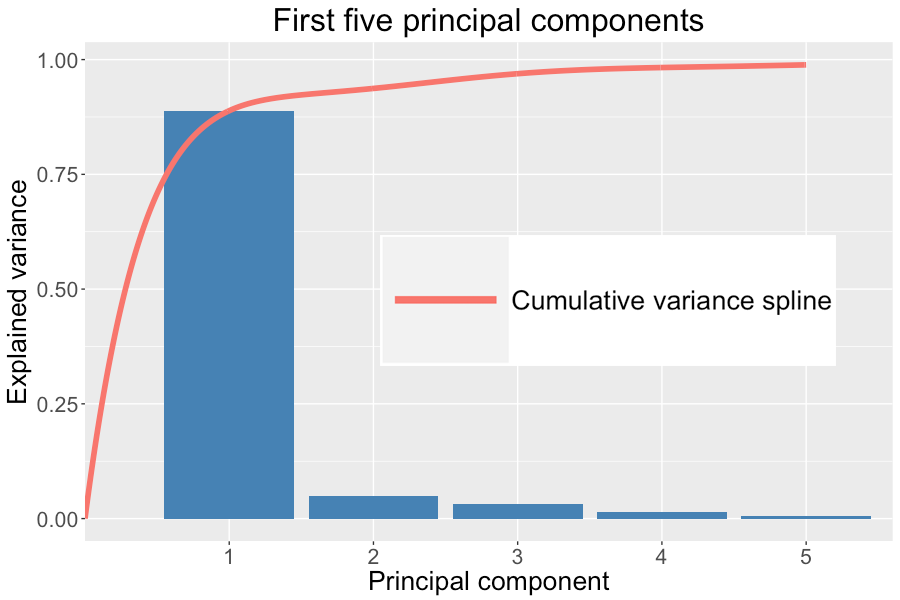
\includegraphics[width=0.6\textwidth]{pca_variance}
    \caption{The blue bars represent the fraction of variance explained by each of the first five principal components. The red is the cumulative amount of variance explained by the first five principal components, interpolated between the bars to form a smooth curve}
  \label{fig:pca_variance}
\end{figure}

In addition to the features based on micromechanical fields, an additional feature is considered based purely on the geometrical configuration of the microstructure.  Experimental data (both from this work and reported throughout the literature) suggest that microstructurally small fatigue-cracks behave much differently near grain boundaries than within a single grain.  It is postulated that the fatigue-crack investigated in this work could have been influenced by certain field variables when near a grain boundary, and others when far from a grain boundary.  To account for such spatially dependent correlation, an additional feature called $d_{GB}$, which is the distance from a given point to the nearest grain boundary, is added to each PCA 3-vector to produce a 4-vector.  This 4-vector is called a descriptor, and is used as the ``raw'' representation from which the fracture surface is inferred.

\section{General strategy}
\index{Error metrics}
\index{Error metrics ! Root mean squared error}
\index{Error metrics ! $R^2$}
Once the data are preprocessed, the objective is to train a machine-learning model to infer the crack surface as a function of the descriptor described above.  As a first attempt, a simple prediction/propagation strategy is implemented.  This strategy is model-agnostic, and will be described without mentioning the specific models chosen.  The entire crack surface described in the previous chapter is split into two equal halves, the front half (the half containing the nucleation point of the crack) and the back half.  The front half of the surface is used to train the machine-learning model, and the back half is predicted using the trained model. The predicted surface is validated by comparing to the known crack surface on the back half of the sample.  The prediction for a single data point is defined as follows:

\begin{enumerate}
  \item For a given point on the current crack surface, take all descriptors within the $\Delta x \times \Delta y \times \Delta z \mu m$ region centered at this point.  Since the microstructure is discretized onto a grid with $1 \mu m$ spacing, this region will contain $\Delta x \times \Delta y \times \Delta z$ descriptors.
  \item Flatten these descriptors into a feature vector of length  $4 \times \Delta x \times \Delta y \times \Delta z$.
  \item Given a feature vector, use the trained model to predict the relative z-offset to the next point in the x-direction (assumed as the approximate growth direction of the crack).
  \item Use a radial basis function (RBF) smoothing spline to ensure that rows of predicted points form a smooth surface.  The purpose of the spline is to bring the values of independently predicted adjacent points closer together.  This spline is used in addition to the predicted values, and is part of the entire machine learning pipeline.  It can be thought of as a type of prior, ensuring that adjacent independently-predicted points on the crack surface do not diverge in a physically unrealistic manner.
\end{enumerate}

Here, the response variable is the z-offset, which represents the vertical distance by which the crack deviates from its current position during propagation.  Specifically, the z-offset for a particular point on the crack surface is the signed vertical distance between itself and the next point in the positive x-direction.  Since the crack surface is assumed to emulate an injective function $f(x, y)$, the problem of predicting the shape of the crack surface is reduced down to predicting the z-value for a given point $(x, y)$.  If the z-offset is predicted for the point $\{x, y\}$ then the z-value for the point $\{x + 1, y\}$ can be calculated by adding the predicted z-offset to the z-value of the point $\{x, y\}$.

The features used for prediction are the descriptors for the points belonging to a region surrounding the point for which the z-offset is being predicted.  The size of this region is a hyperparameter that is modified during model comparison, the largest attempted value being $10 \mu m \times 10 \mu m \times 10 \mu m$ (such a region produces $10 \times 10 \times 10 \times 4 = 4000$ features for a given point).

Because the prediction of a particular point requires the known value of the prior crack surface point, the prediction methodology implemented here closely emulates the actual sequence of crack evolution in a physical sample.  To better understand this, consider that the model has trained on all points in the crack surface from $0 ... n$, where $n$ is the halfway point in the x-direction.  At the beginning of the testing phase, the model uses the feature vectors associated with the points at $n$ to predict the z-positions of the points at $n + 1$.  Then, the feature vectors associated with the predicted z-positions for the points at $n + 1$ are used to predict the z-positions of the points at $n + 2$.  This continues until the entire crack surface had been predicted.

While errors can potentially propagate throughout the testing phase due to dependence on previous predictions, this prediction strategy closely mirrors the actual real-world use case for predicting crack growth.  Specifically, the model needs to be able to perform well under the assumption that large portions of the crack surface are unknown, where the most common case is when the unknown portions are in the path of future crack growth.

Both $R^2$ and root mean squared error (RMSE) are used as error metrics and are calculated by using the difference in actual and predicted z-values.  The difficulty in measuring model accuracy for this strategy is that predicted points closer to the training points generally have lower errors, while predicted points farther from the training points had higher errors.  While using the $R^2$ and RMSE for all testing points helps combat this problem, there is still a need for a sense of relative success of the model.  Therefore, much like in the last chapter, a hypothetical crack surface is created against which predicted crack surfaces are compared.  This hypothetical crack surface simply uses the z-values of the crack surface points where the training data ended, and extends those z-values forward in the x-direction.  This is the most sensible approach, since the distribution of relative z-offsets is a normal distribution with mean zero, as shown in Figure \ref{fig:distribution}.

\begin{figure}[b]
  \centering
    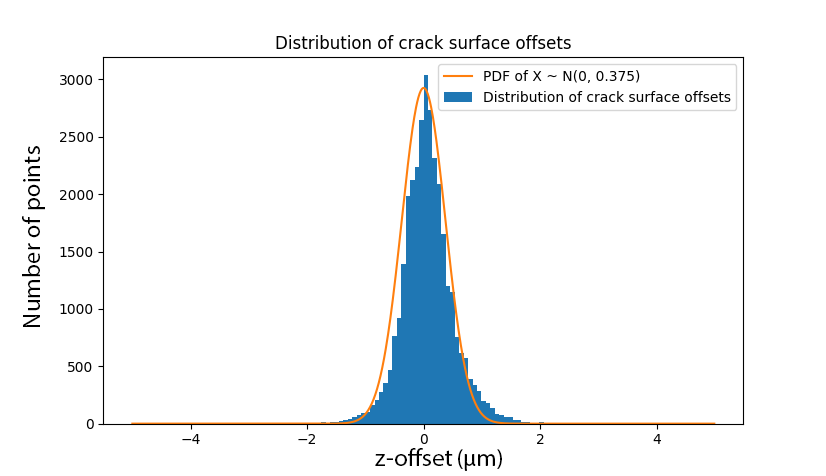
\includegraphics[width=0.7\textwidth]{distribution}
    \caption{Histogram of the distribution of z-offset values}
  \label{fig:distribution}
\end{figure}

To provide further comparison, a simpler set of features is also investigated.  Instead of using the PCA 3-vector described above, the descriptor for comparison contains simply the Euler angles representing the grain orientation at each point.  This is a worthwhile exercise, in that Euler angles are intrinsic properties of the material whose acquisition requires no simulation, as described in Chapter 3.  The rationale behind using the Euler angles as features is to assess how well the model can predict crack growth without load-dependent features such as stress and strain.  As before, $d_{GB}$ is appended to each 3-vector to produce a 4-vector.

\section{Crack surface height inference}
\index{Artificial neural network ! Convolutional}
\index{Random forest}
\index{Support vector machine}
In this work, two machine-learning models are considered for the prediction of the response variable.  The first chosen model is a convolutional neural network (CNN), in accordance with the assumption that spatial-relation based algorithms might perform well on this representation of the data.  The CNN is implemented by the Keras library for Python \cite{keras}.  The structure of the CNN is shown in Figure \ref{fig:cnn}.

\begin{figure}[b]
  \centering
    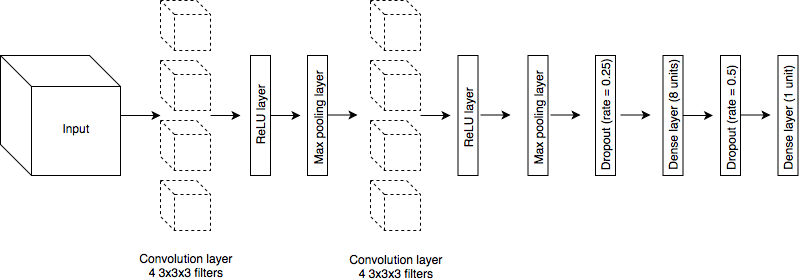
\includegraphics[width=0.7\textwidth]{cnn}
    \caption{Structure of the convolutional neural network used in this chapter}
  \label{fig:cnn}
\end{figure}

The CNN was trained for either 5 or 10 epochs.  Beyond 10 epochs, the model did not improve much, and was at risk for overfitting.  The second chosen model is the XGBoost library \cite{xgboost}, which uses a random forest based model.  This model contains many default parameters, but the most significant are likely the number of trees (100) and maximum tree depth (6).

Table \ref{table:model-comparison} compares the results of each model.  Figure \ref{fig:surfaces} shows the resulting surface for a selection of the rows from the table.  The front half of the crack surface is constant in all images, since it was treated as ``known'' and used as the training data.  The back half is different across all images, and represents the area predicted by the model.

\begin{table}[t]
  \centering
  \caption{Crack surface height inference results for each chosen model}
  \label{table:model-comparison}
  \begin{tabular}{| c | c | c | c | c | c | c |} \hline
    \textbf{Model} & \textbf{Features} & \textbf{XY-distance} & \textbf{Z-distance} & \textbf{Epochs} & $\bm{R^2}$     & \textbf{RMSE}           \\ \hline
    CNN            & PCA vectors       & 10 $\mu m$           & 10 $\mu m$          & 10              & \textbf{0.891} & \textbf{10.156} $\mu m$ \\ \hline
    CNN            & PCA vectors       & 10 $\mu m$           & 10 $\mu m$          & 5               & \textbf{0.789} & \textbf{14.131} $\mu m$ \\ \hline
    CNN            & Euler angles      & 10 $\mu m$           & 10 $\mu m$          & 10              & \textbf{0.844} & \textbf{12.156} $\mu m$ \\ \hline
    XGBoost        & PCA vectors       & 10 $\mu m$           & 10 $\mu m$          & N/A             & \textbf{0.888} & \textbf{10.314} $\mu m$ \\ \hline
    XGBoost        & PCA vectors       & 6  $\mu m$           & 6  $\mu m$          & N/A             & \textbf{0.875} & \textbf{10.873} $\mu m$ \\ \hline
    XGBoost        & Euler angles      & 10 $\mu m$           & 10 $\mu m$          & N/A             & \textbf{0.669} & \textbf{17.690} $\mu m$ \\ \hline
    \multicolumn{5}{|c|}{Hypothetical crack surface}                                                  & \textbf{0.788} & \textbf{14.168} $\mu m$ \\ \hline
  \end{tabular}
\end{table}

\begin{figure}[b]
  \centering
    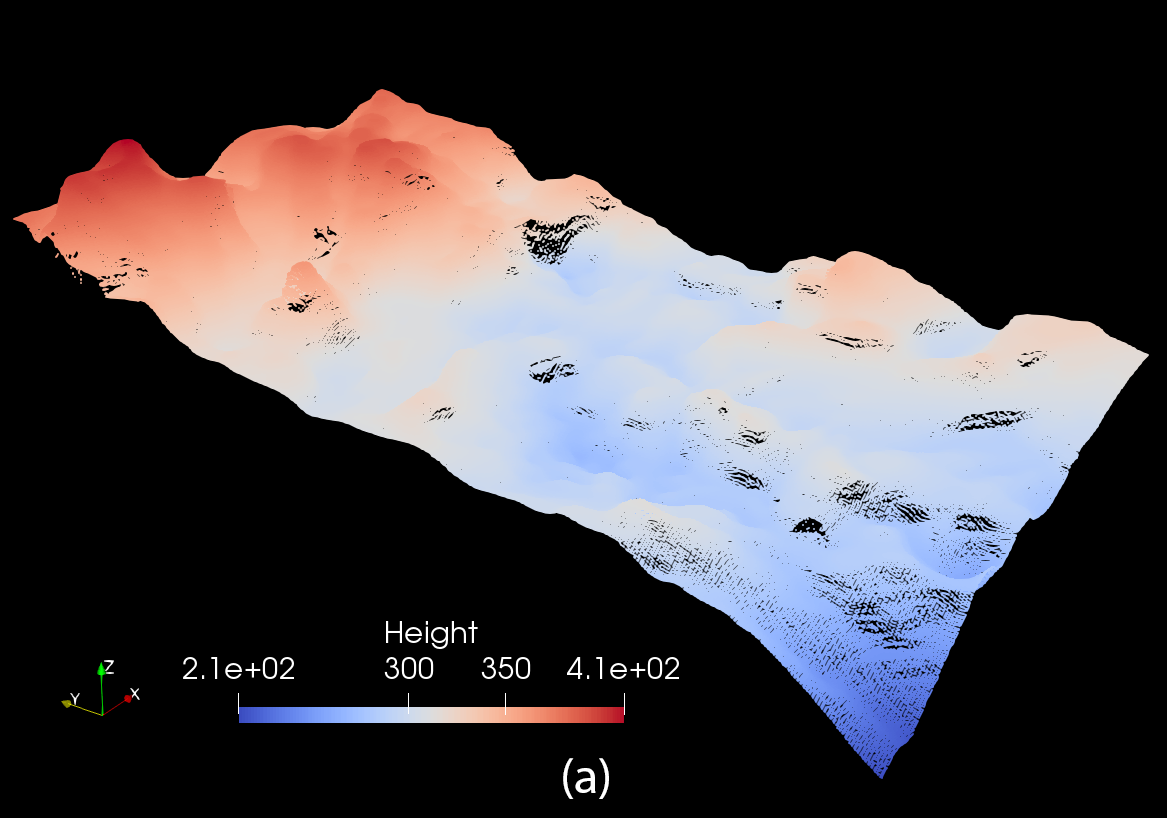
\includegraphics[width=0.42\textwidth]{surface_actual} %a
    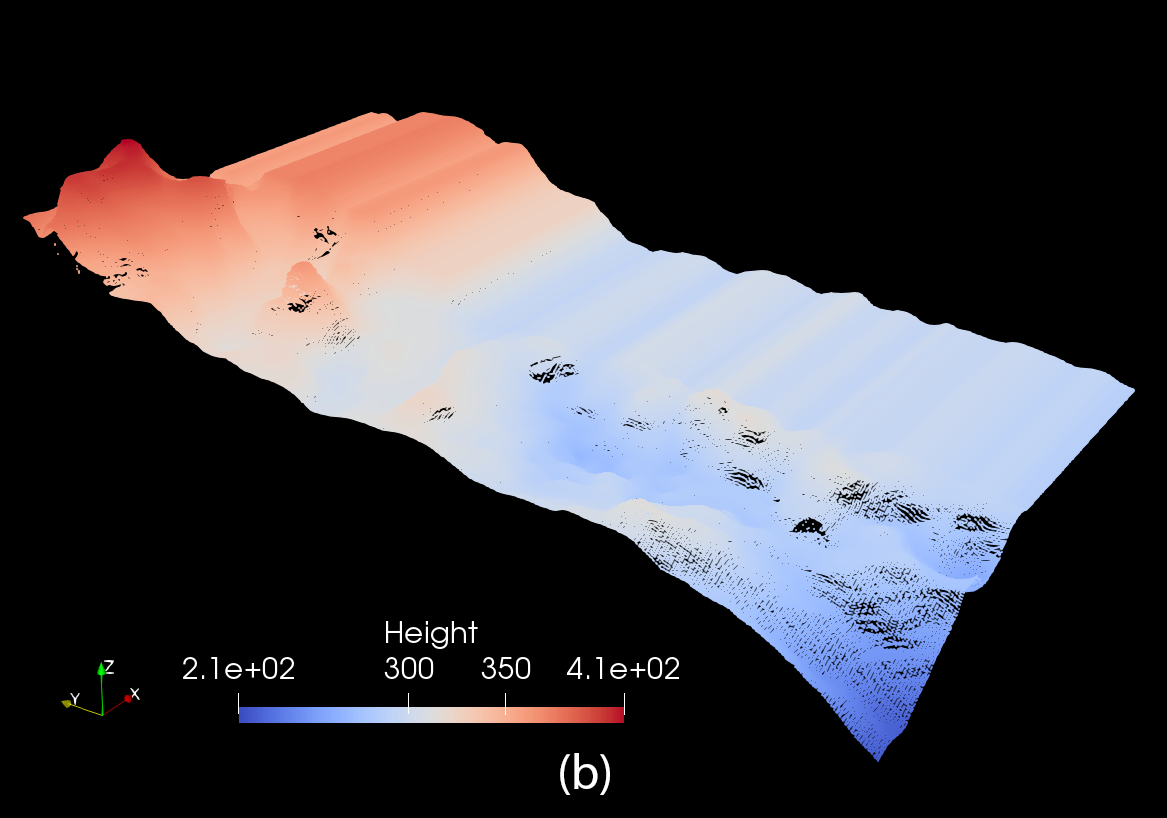
\includegraphics[width=0.42\textwidth]{surface_control} %b
    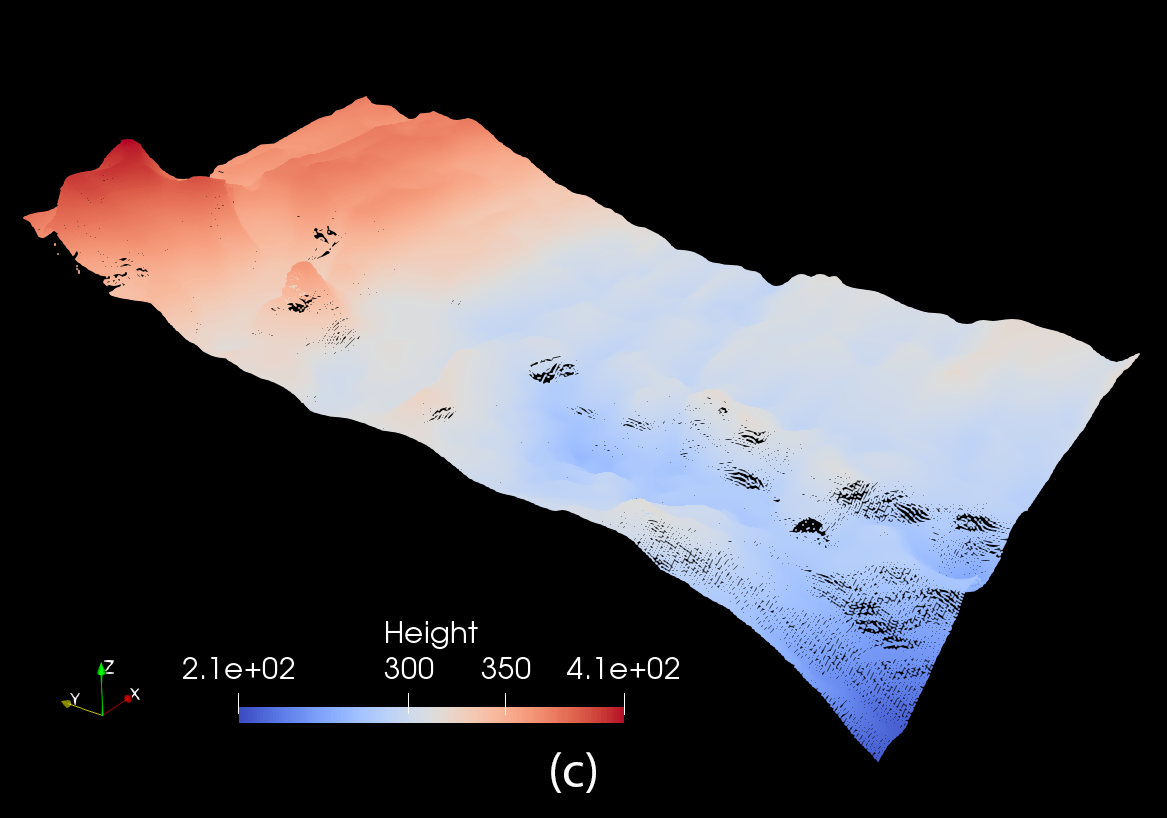
\includegraphics[width=0.42\textwidth]{surface_cnn_pca_10_10} %c
    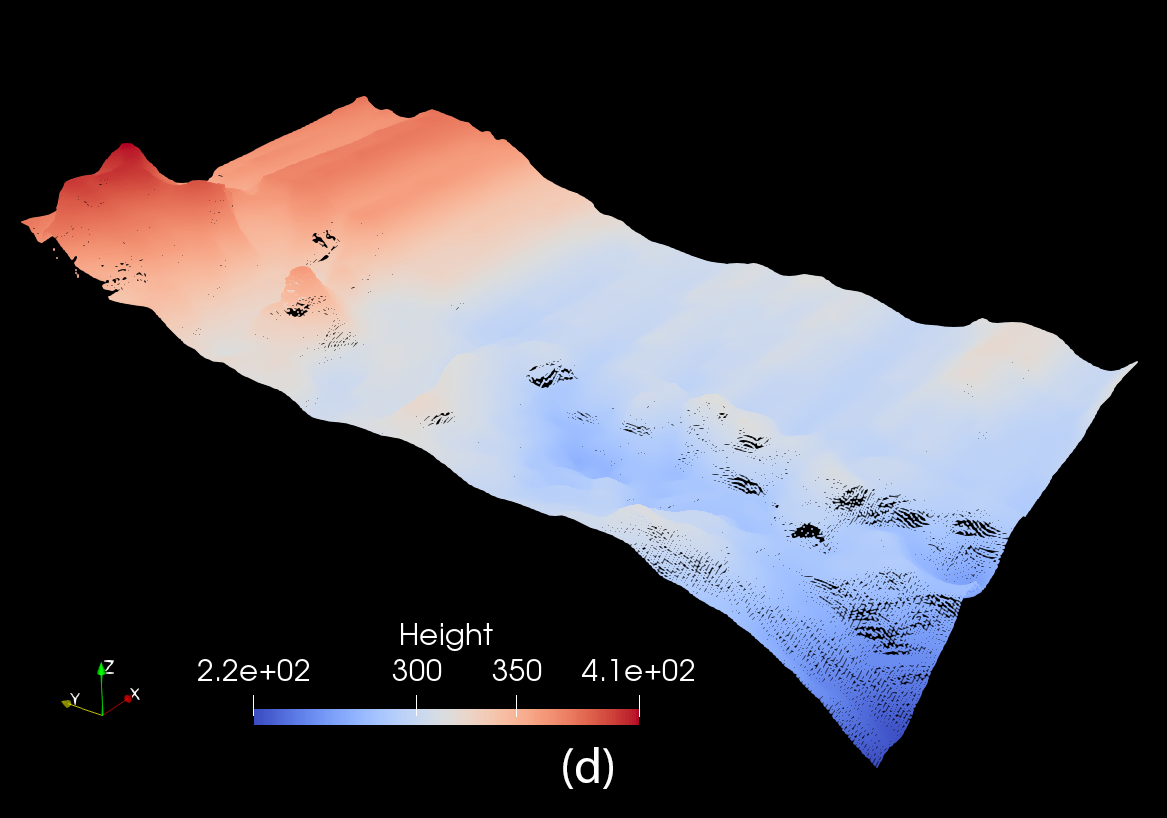
\includegraphics[width=0.42\textwidth]{surface_cnn_pca_10_10_5} %d
    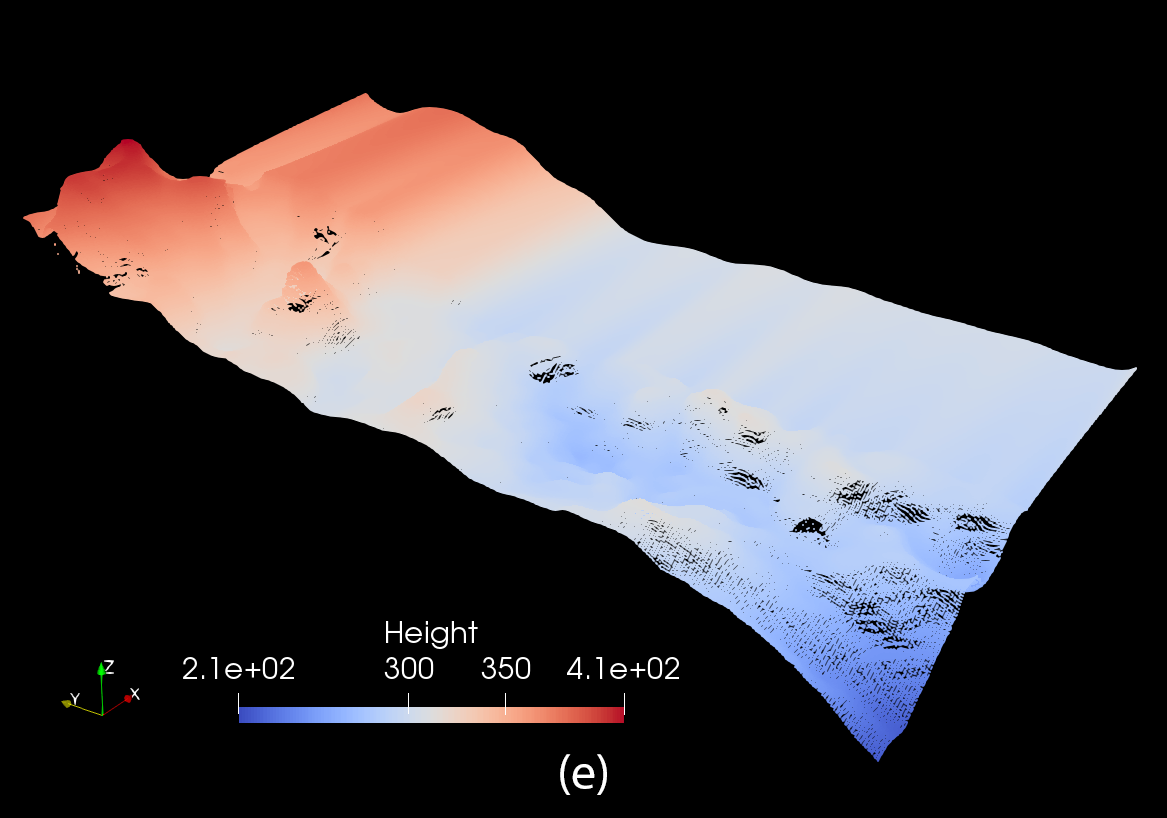
\includegraphics[width=0.42\textwidth]{surface_cnn_euler_10_10} %e
    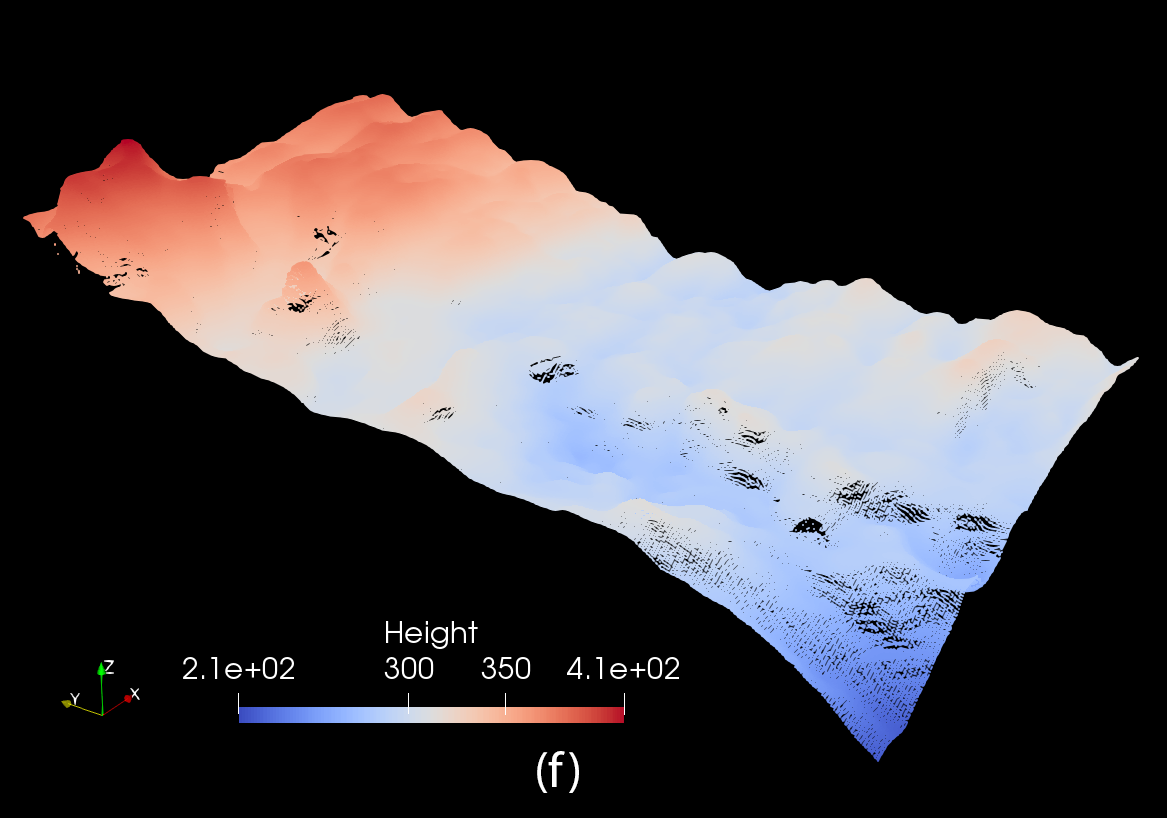
\includegraphics[width=0.42\textwidth]{surface_xgboost_pca_10_10} %f
    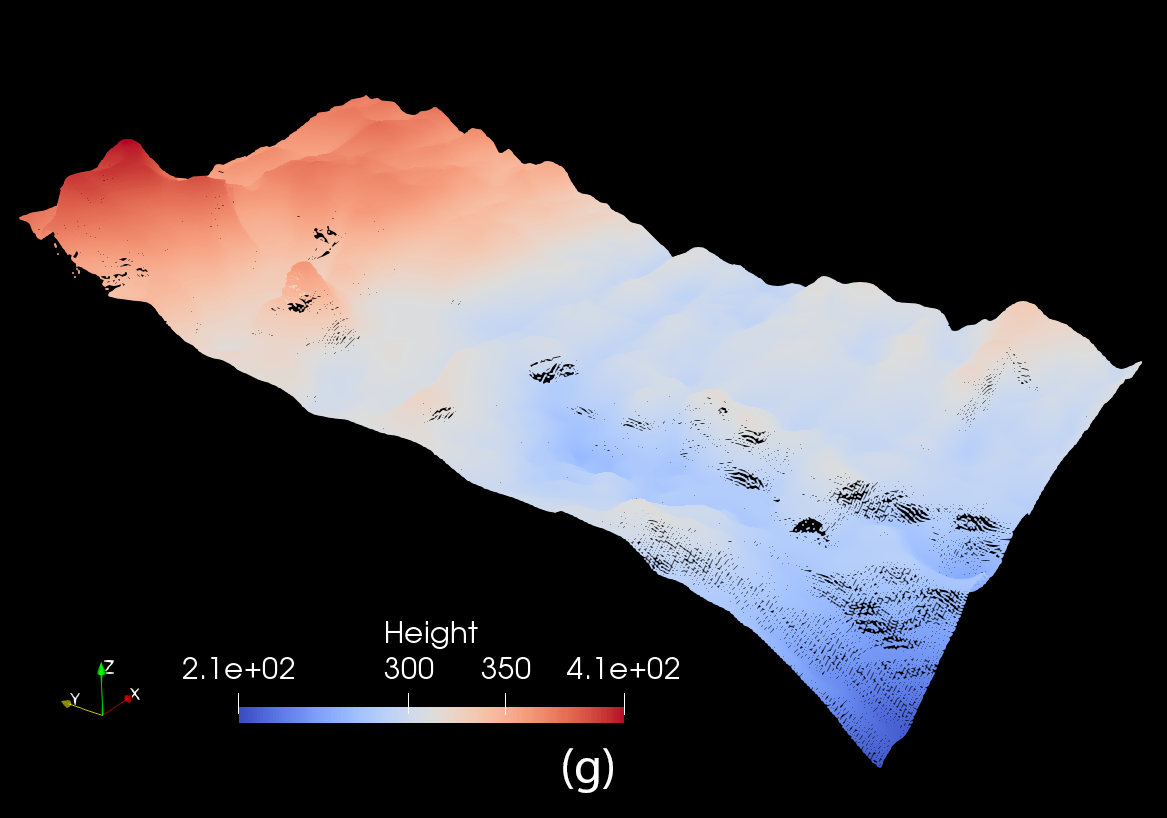
\includegraphics[width=0.42\textwidth]{surface_xgboost_pca_6_6} %g
    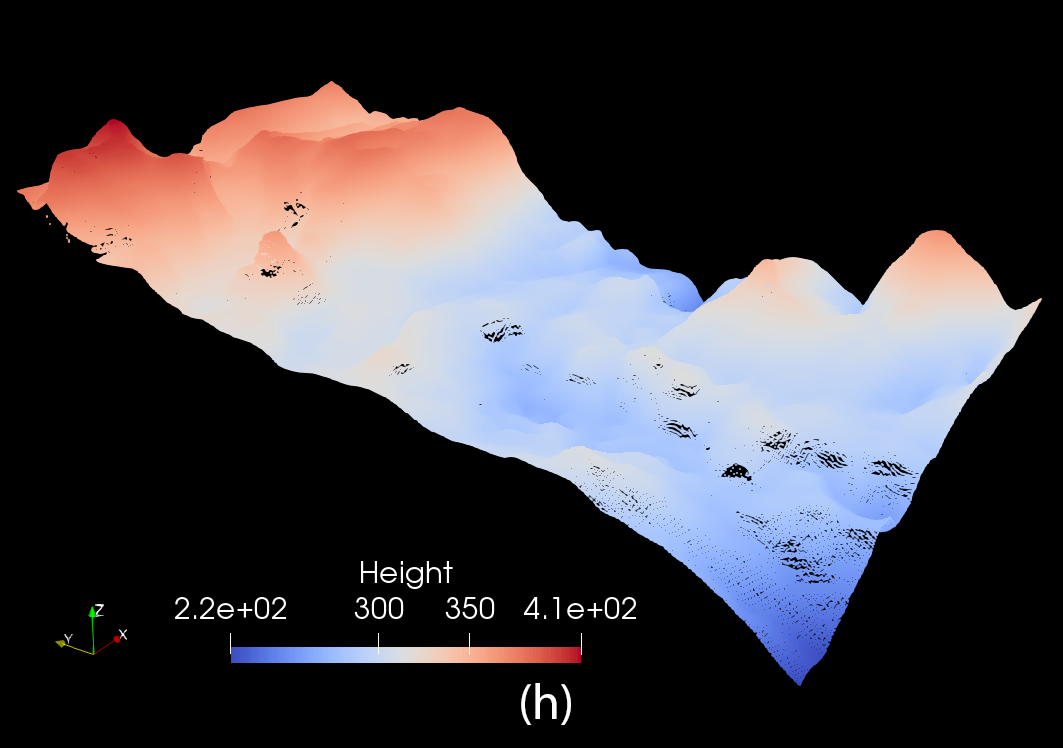
\includegraphics[width=0.42\textwidth]{surface_xgboost_euler_10_10} %h
    \caption{\textbf{Actual and predicted crack surfaces (a)} Actual crack surface
             \textbf{(b)} Hypothetical crack surface
             \textbf{(c)} CNN prediction, using PCA vectors and a $10 \times 10 \times 10 \mu m$ region (trained for 10 epochs)
             \textbf{(d)} CNN prediction, using PCA vectors and a $10 \times 10 \times 10 \mu m$ region (trained for 5 epochs)
             \textbf{(e)} CNN prediction, using Euler angles and a $10 \times 10 \times 10 \mu m$ region (trained for 10 epochs)
             \textbf{(f)} XGBoost prediction, using PCA vectors and a $10 \times 10 \times 10 \mu m$ region
             \textbf{(g)} XGBoost prediction, using PCA vectors and a $6 \times 6 \times 6 \mu m$ region
             \textbf{(h)} XGBoost prediction, using Euler angles and a $10 \times 10 \times 10 \mu m$ region }
    \label{fig:surfaces}
\end{figure}

The base performance achieved by simply ``extending'' the crack surface is shown in the last row of Table \ref{table:model-comparison}.  Notice that most of the trained models surpass this performance, which is promising.  As hypothesized, the CNN seems to be the most accurate in its predictions, as indicated by the first row in the table.  This reaffirms the notion that models which encode spatial relationships in the microstructure are capable of achieving greater success.  When using PCA vectors as features, both models attain higher accuracy than when using Euler angles.  However, this disparity is smaller in the case of the CNN, indicating again that Euler angles are much more meaningful when spatially associated with grains.  This makes sense when considering that the CNN may be learning filters based on the locations of the grain boundaries, which are implicitly encoded in the Euler angles.  Another interesting observation is that decreasing the size of the region from which descriptors are sampled for a given point from $6 \times 6 \times 6$ to $10 \times 10 \times 10$ does not have a huge impact on performance.  This shows that increasing the area gives diminishing returns, which is a useful observation to anyone concerned about computation.

The images show that all models make relatively safe predictions, i.e. that the models are reluctant to predict high z-offset values, which results in smoother surfaces.  This is one area where the chosen prediction strategy is lacking.  Prediction of anomalies is highly unlikely under this particular strategy.

\section[Crack-surface height inference based on a radial prediction strategy]{Crack-surface height inference based on a radial \\ prediction strategy}
Another prediction strategy is implemented that more closely emulates the actual growth behavior of the observed crack.  Rather than training on the front half and propagating towards the back half of the sample in the x-direction, the method presented here trains on a semicircular area emanating outward from the nucleation point of the crack.  The prediction then attempts to expand this area radially outward.  This is done by moving point-wise along a semi-circular ``known'' region of the crack surface (which began as simply the training region) and predicting the z-offset for three of the adjacent points on the xy-plane, as shown in Figure \ref{fig:radial}.  If any of the z-values for these points are already known, the predicted value is ignored.  Otherwise, the predicted value is used to produce a z-coordinate for the point.  If the predictions of multiple known points overlap, then the mean of all predictions is taken.  Once a prediction for the z-coordinate is produced, the point is added to the known region.  This continues until the z-coordinates of all points within the area of the final crack front have been predicted.

\begin{figure}[b]
  \centering
    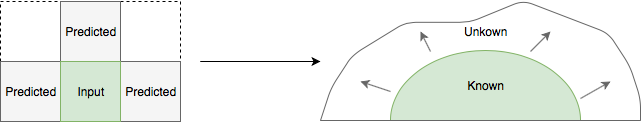
\includegraphics[width=0.7\textwidth]{radial}
    \caption{Visualization of the radial prediction strategy.  On the left is shown the points for which the predicted z-values of a single point correspond.  On the right is the desired effect of this prediction strategy.}
  \label{fig:radial}
\end{figure}

The benefit of this strategy is that it more closely resembles the actual shape of the experimentally observed crack fronts.  An additional benefit of this approach is that fatigue-crack growth rate, $\frac{da}{dN}$, was previously parameterized in the same manner (viz., along radial paths from the nucleation site). Consequently, $\frac{da}{dN}$ could be considered in future work as the prediction metric to complement the prediction of crack-surface height.

The wedge prediction strategy from Chapter 2 is also implemented here, as it has merit in inferring portions of the crack surface where measurements are produced with high levels of uncertainty.  In this case, the area containing the crack fronts is split into $6$ wedges of equal angular degree, and the 3 wedges that contain the highest percentage of uncertain data are used as the testing portions.  A selection of the results for models predicting z-offset are given in Table~\ref{table:radial-comparison}, with images given in Figure \ref{fig:radial_predictions}.  For comparison, SVR is used as one of the models, since it had been used in a similar fashion in Chapter 2.

\begin{table}[b]
  \centering
  \caption{Crack surface height inference results for each chosen model, using a radial propagation strategy}
  \label{table:radial-comparison}
  \begin{tabular}{| c | c | c | c | c | c | c |} \hline
    \textbf{Model} & \textbf{Features} & \textbf{XY-distance} & \textbf{Z-distance} & \textbf{Split}  & $\bm{R^2}$     & \textbf{RMSE}           \\ \hline
    XGBoost        & PCA vectors       & 10 $\mu m$           & 10 $\mu m$          & Radial          & \textbf{0.784} & \textbf{9.344}  $\mu m$ \\ \hline
    XGBoost        & PCA vectors       & 10 $\mu m$           & 10 $\mu m$          & Wedge           & \textbf{0.579} & \textbf{12.216} $\mu m$ \\ \hline
    SVR            & PCA vectors       & 10 $\mu m$           & 10 $\mu m$          & Radial          & \textbf{0.653} & \textbf{11.049} $\mu m$ \\ \hline
    SVR            & PCA vectors       & 10 $\mu m$           & 10 $\mu m$          & Wedge           & \textbf{0.572} & \textbf{12.312} $\mu m$ \\ \hline
  \end{tabular}
\end{table}

\begin{figure}[t]
  \centering
    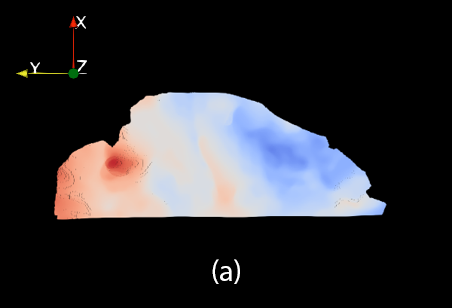
\includegraphics[height=0.22\textwidth]{radial_actual}
    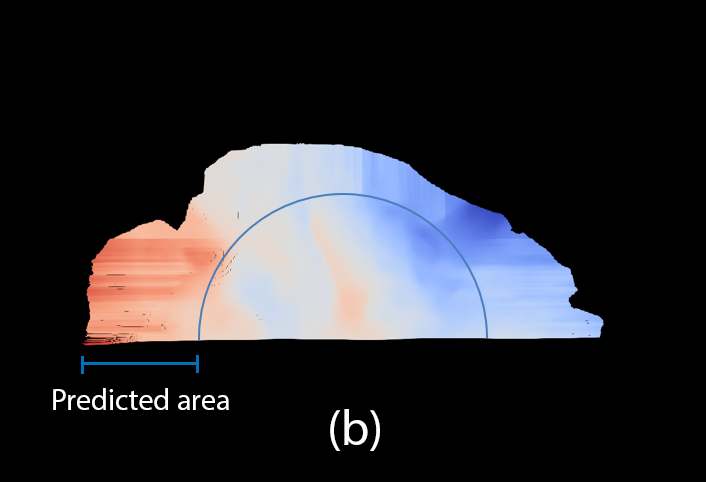
\includegraphics[height=0.22\textwidth]{radial_xgboost}
    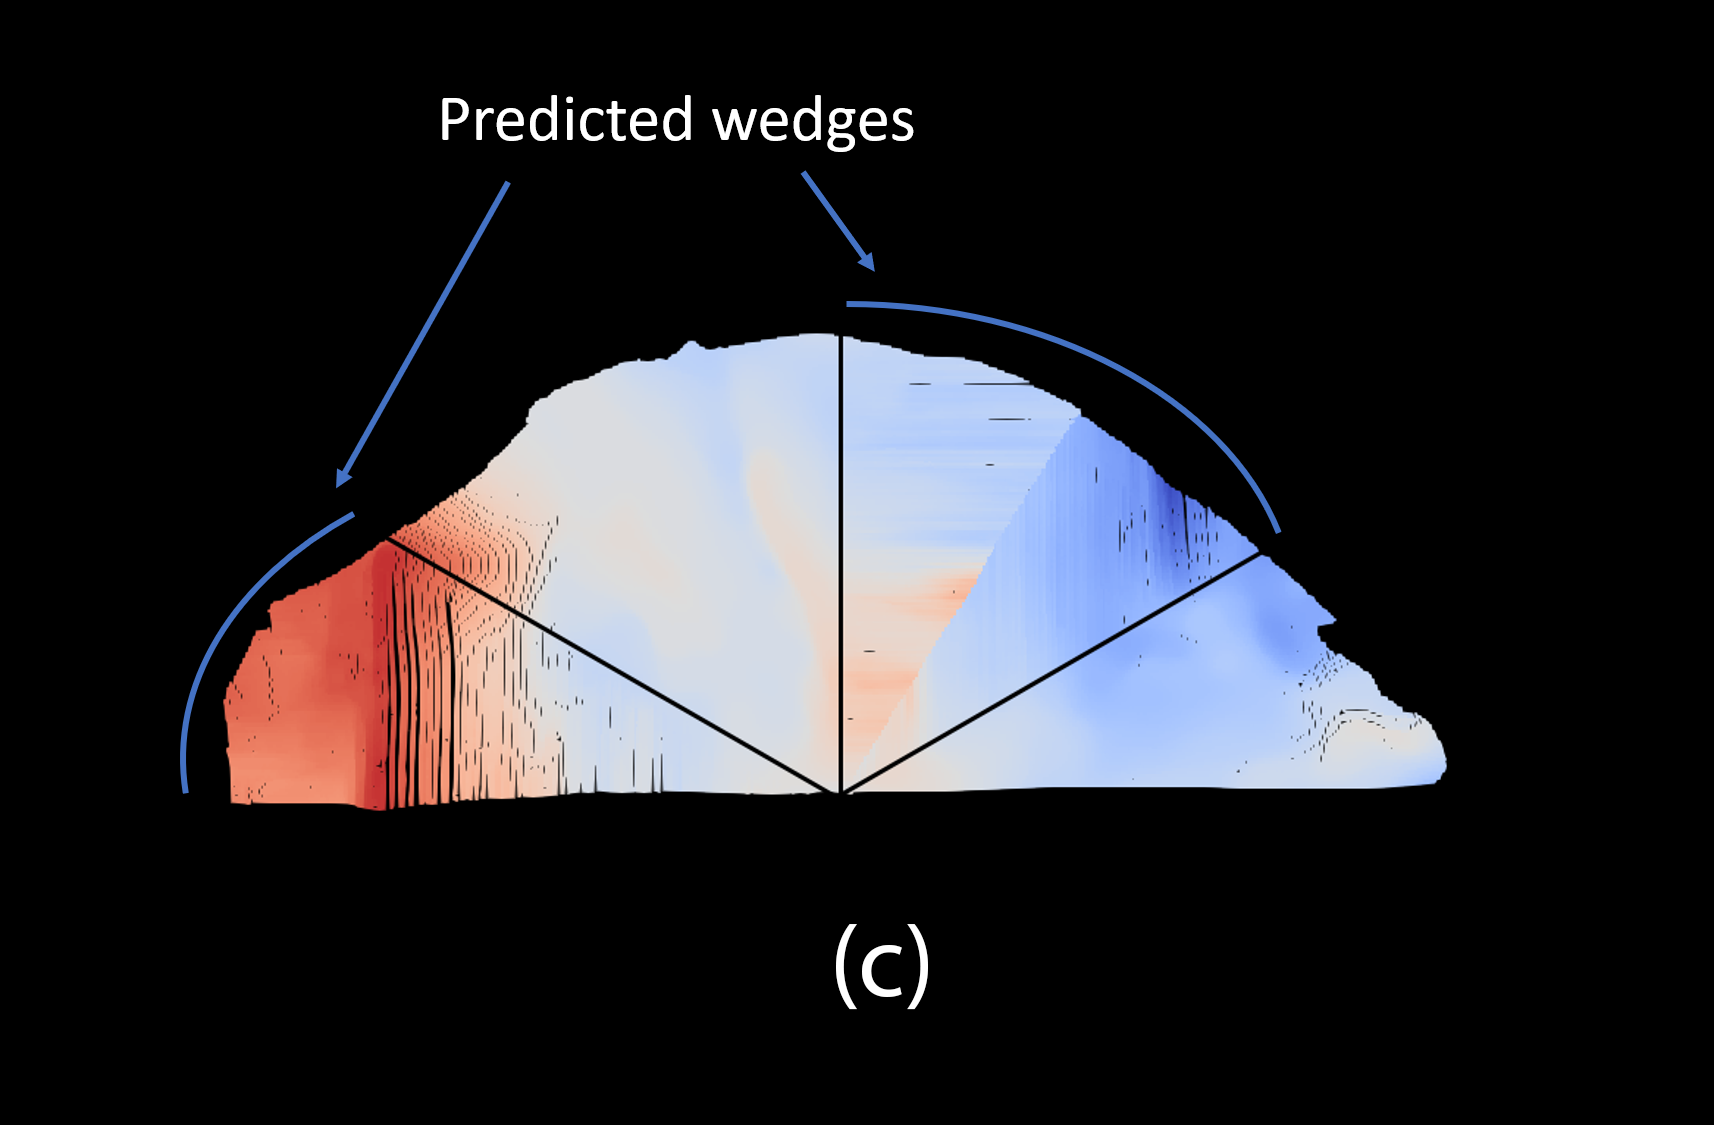
\includegraphics[height=0.22\textwidth]{wedge_xgboost}
    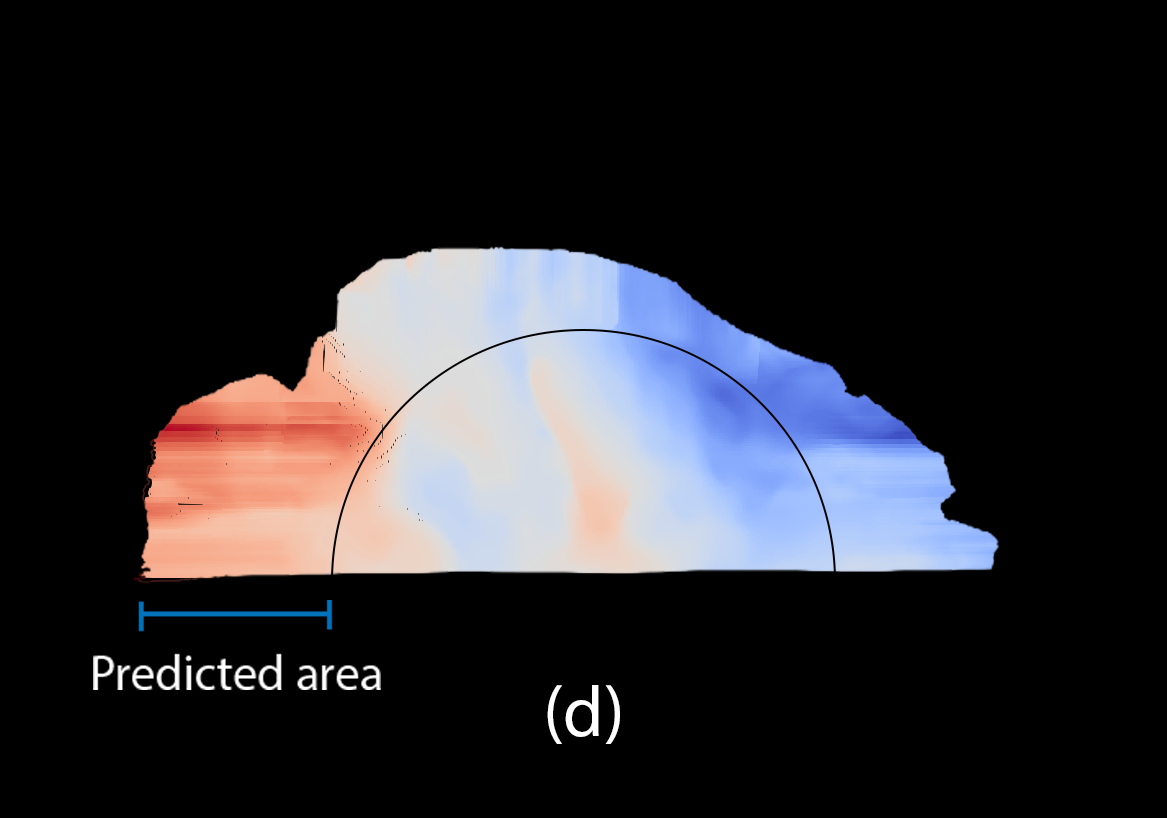
\includegraphics[height=0.22\textwidth]{radial_svr}
    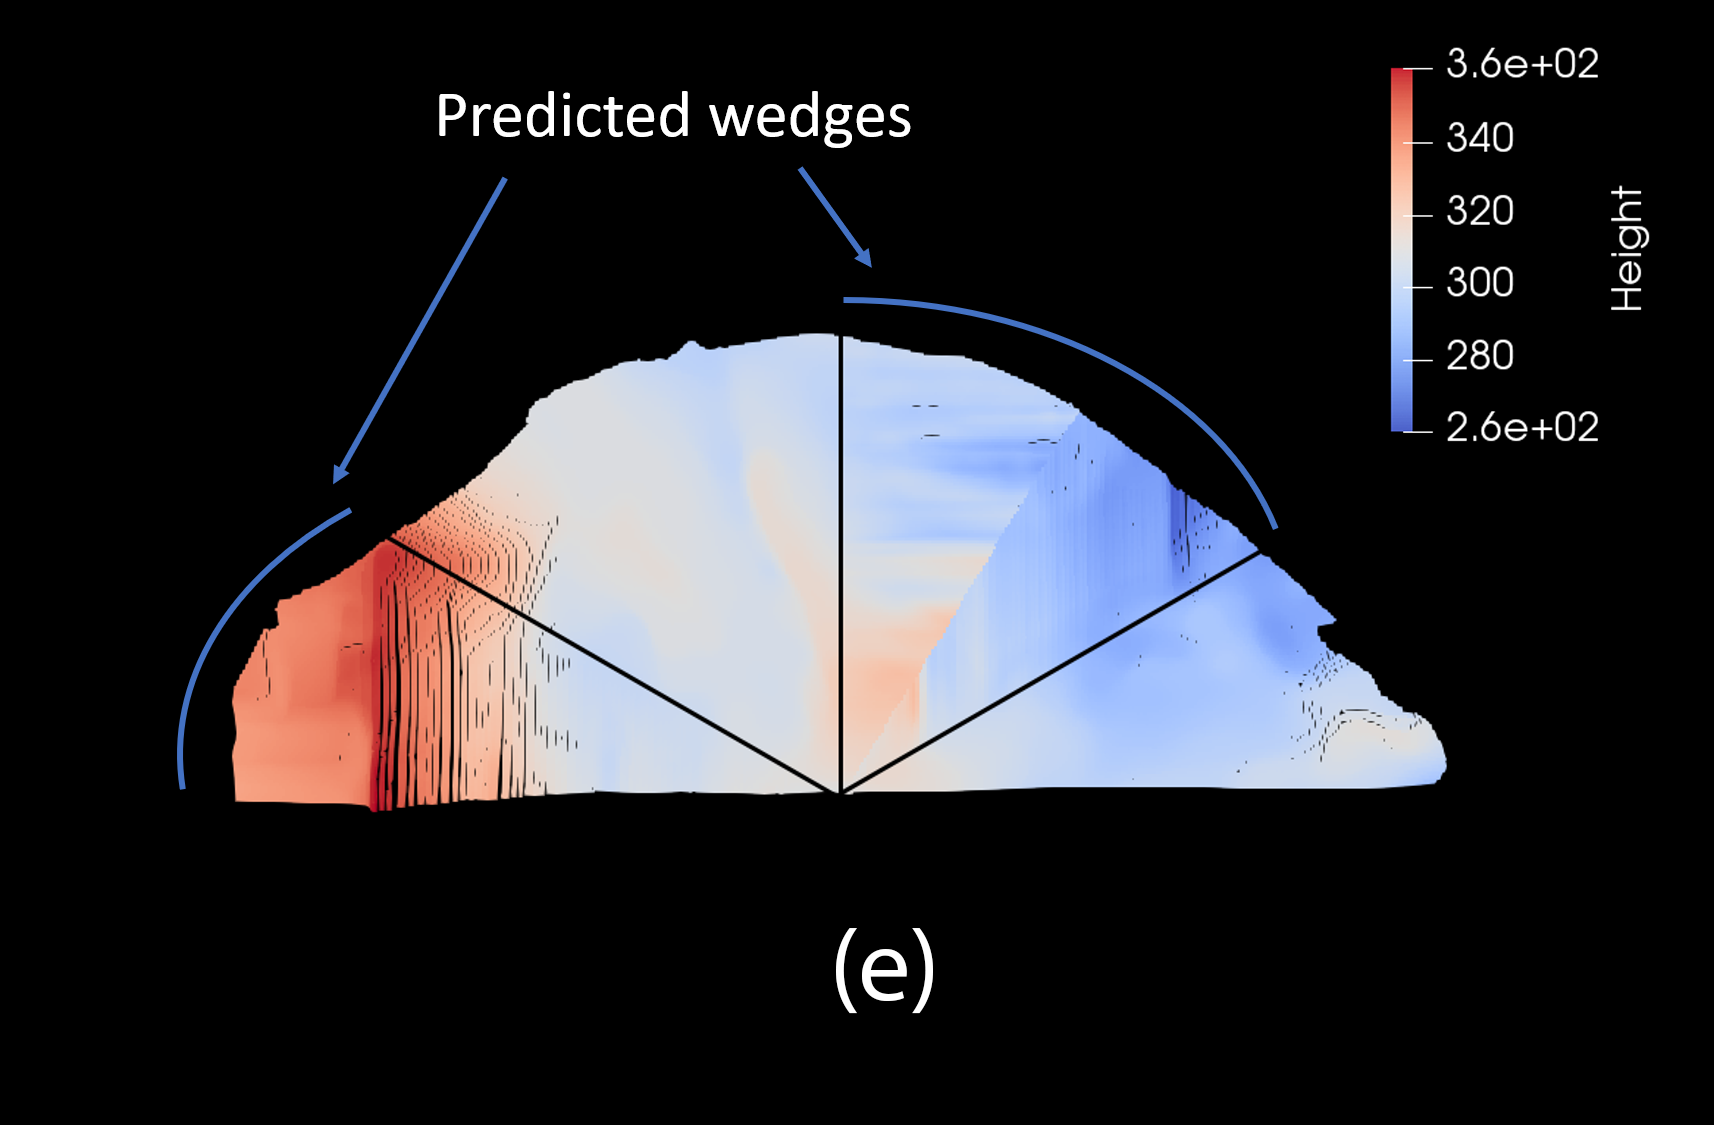
\includegraphics[height=0.22\textwidth]{wedge_svr}
    \caption{\textbf{Actual and predicted radial crack surfaces (a)}  Actual crack surface.
             \textbf{(b)} XGBoost prediction, using a radial propagation strategy
             \textbf{(c)} XGBoost prediction, using a wedge propagation strategy
             \textbf{(d)} SVR prediction, using a radial propagation strategy
             \textbf{(e)} SVR prediction, using a wedge propagation strategy
             Each of these predictions have been cropped to the shape of the measured crack surface inside of the final crack front. }
  \label{fig:radial_predictions}
\end{figure}

Interestingly, the wedge strategy performs poorly in both test cases.  This is likely because the prediction strategy does not follow the actual direction of crack growth, and so predicted z-values are dependent of points that may not have chronologically preceded the predicted point.  The XGBoost library outperforms SVR in both cases, suggesting that the actual crack growth function is highly nonlinear.

\section{Conclusion}
The results from this chapter are much more promising than those of Chapter 2.  Nearly all of the z-offset predictions are better using a trained model vs. using the hypothetical crack surface.  This shows that the trained model is more successful than not when making predictions about which direction that crack will grow.  In some cases, the improvement is quite significant, reaching up to a $12.69\%$ improvement in $R^2$ and a $27.20\%$ improvement in RMSE the optimal case (row 1 of Table \ref{table:model-comparison}).  Not only does this mean that the machine-learned models are capable of making relatively accurate short-term predictions, but also that they can minimize and even correct the propagation of errors in long-term predictions.

While the z-offset predictions seem meaningful, their usefulness remains unknown.  Without more data, it is difficult to know how the number of training points can affect the results, as well as how long the prediction strategy can remain accurate before small errors begin to cause large deviations.  It is also difficult to determine how well this strategy generalizes to other cracks, i.e. if the training data from one crack can be used to predict the results of a completely different crack.  Additionally, without the associated $\frac{da}{dN}$ information, it is impossible to know when the crack will grow to the various predicted locations.  Still, knowing approximately where the crack will grow can be useful for determining when it might start to compromise the integrity of the material.

One of the drawbacks of using sophisticated machine learning methods is lack of interpretability.  There are ways of analyzing certain aspects of the model to get an idea of what influences its decisions.  For a CNN, this could mean examining the learned convolutional filters, whereas for a random forest, this could mean looking at which features are used as the root node in the majority of trees.  However, when the CNN has multiple layers and thousands of filters, this can be challenging.  Even in less complicated models, if PCA representations are used for features, any interpretation of how the original features relate to the response variable becomes much more challenging.

Predicting $\frac{da}{dN}$ remains a difficult problem.  This is partly due to the few number of data points, as well as the limited number of unique crack fronts.  Additionally, the extracted features are more prone to being relevant to crack point location, since the correlations were calculated with respect to distance to crack surface.  Thus, the success of the z-offset predictions is actually quite promising for the potential success of $\frac{da}{dN}$ predictions.  Under a different feature selection strategy, the pipeline presented in this chapter might achieve comparable success with $\frac{da}{dN}$ predictions.

Future work might explore these feature selection strategies, as well as incorporate more data.  Having multiple instances of fatigue-cracks would be very useful in training models that generalize well.  Beyond this, a challenging remaining problem is the prediction of anomalies in the crack surface.  A data split that isolated these anomalies to see how well they could be predicted would be an interesting and enlightening endeavor.

\bibliographystyle{ieeetr}
\bibliography{\jobname}
